% Bagian Hasil Percobaan
\section*{Hasil Percobaan} % Jika ada hasil percobaan

Hasil percobaan yang diperoleh adalah sebagai berikut:

\begin {enumerate}
    \item Percobaan 1: Point-to-Point
    
    Dari hasil konfigurasi yang telah dilakukan, didapatkan IP Address pada masing-masing router sebagai berikut:

    \begin{tcolorbox}[colframe=blue, colback=lightgray, title=Router 1]
    IP Address: 20.20.20.2
    \end{tcolorbox}

    \begin{tcolorbox}[colframe=blue, colback=lightgray, title=Router 2]
        IP Address: 20.20.20.3
    \end{tcolorbox}
    
    Hasil pengujian Point-to-Point dapat dilihat pada Gambar \ref{fig:router1_pengujian1} dan Gambar \ref{fig:router2_pengujian1}. Dari hasil pengujian tersebut, dapat dilihat bahwa kedua router dapat terhubung dengan baik dengan melakukan \textit{ping} dari router 1 ke router 2 dan sebaliknya.

    \begin{figure}[H]
        \centering
        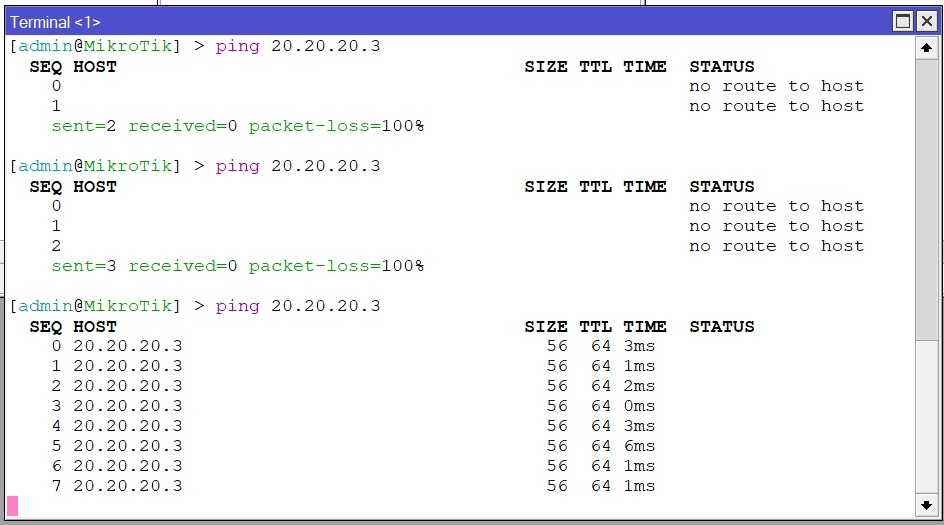
\includegraphics[width=0.6\textwidth]{img/router_1_pengujian1.jpeg}
        \caption{Hasil Pengujian Point-to-Point pada Router 1}
        \label{fig:router1_pengujian1}
    \end{figure}

    \begin{figure}[H]
        \centering
        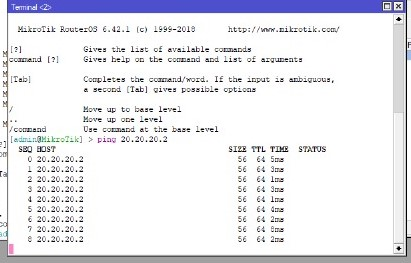
\includegraphics[width=0.6\textwidth]{img/router_2_pengujian1.jpeg}
        \caption{Hasil Pengujian Point-to-Point pada Router 2}
        \label{fig:router2_pengujian1}
    \end{figure}

    \item Percobaan 2: Point-to-Multipoint
    
    Dengan menggunakan IP Address yang sama dengan percobaan 1, hasil pengujian Point-to-Multipoint dapat dilihat pada Gambar \ref{fig:router1_pengujian2} dan Gambar \ref{fig:router2_pengujian2}. Dari hasil pengujian tersebut, dapat dilihat bahwa kedua router dapat terhubung dengan baik dengan melakukan \textit{ping} dari router 1 ke router 2 dan sebaliknya.

    \begin{figure}[H]
        \centering
        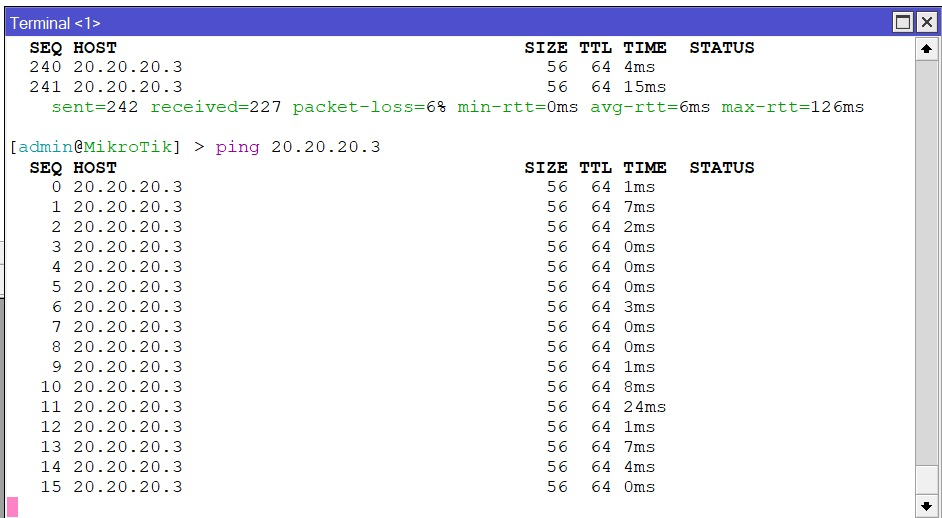
\includegraphics[width=0.6\textwidth]{img/router_1_pengujian2.jpeg}
        \caption{Hasil Pengujian Point-to-Multipoint pada Router 1}
        \label{fig:router1_pengujian2}
    \end{figure}

    \begin{figure}[H]
        \centering
        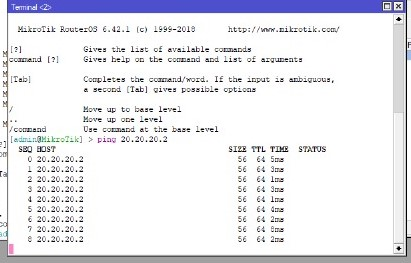
\includegraphics[width=0.6\textwidth]{img/router_2_pengujian1.jpeg}
        \caption{Hasil Pengujian Point-to-Multipoint pada Router 2}
        \label{fig:router2_pengujian2}
    \end{figure}
    
    \item Percobaan 3: Wireless Bridging
    
    Hasil pengujian Wireless Bridging dapat dilihat pada Gambar \ref{fig:router1_pengujian3} dan Gambar \ref{fig:router2_pengujian3}. Dari hasil pengujian tersebut, dapat dilihat bahwa kedua router dapat terhubung dengan baik dengan melakukan \textit{ping} dari router 1 ke router 2 dan sebaliknya.

    \begin{figure}[H]
        \centering
        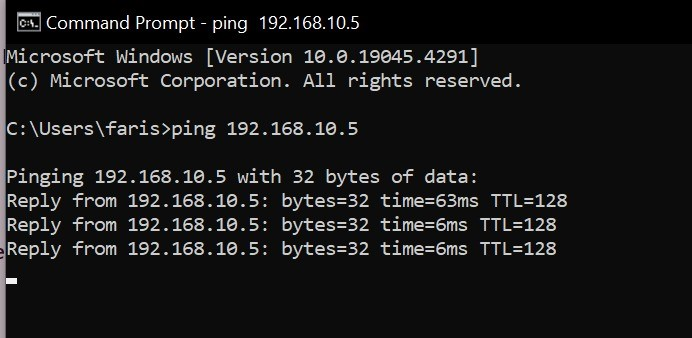
\includegraphics[width=0.6\textwidth]{img/router_1_pengujian3.jpeg}
        \caption{Hasil Pengujian Wireless Bridging pada Router 1}
        \label{fig:router1_pengujian3}
    \end{figure}

    \begin{figure}[H]
        \centering
        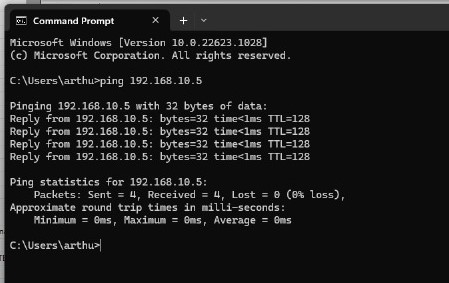
\includegraphics[width=0.6\textwidth]{img/router_2_pengujian3.jpeg}
        \caption{Hasil Pengujian Wireless Bridging pada Router 2}
        \label{fig:router2_pengujian3}
    \end{figure}


\end {enumerate}